\section{The Visualization Composer}
\label{sec:composer}

Our goal is to design a web-based system that facilitates interactive manipulation and customization of visualizations. For the sake of simplicity, we describe our visualization composer by using the notations of Javascript. We employ the rules of SVG elements in HTML5 as the graphical primitives which encode data with visual properties, such as shape, path, size, color, position, transparency and orientation. The primitives can be inherited and extended to construct complicated forms.
%Basic primitives can be classified into three categories: shapes ( \emph{Line},  \emph{Circle}, \emph{Rect}, \emph{Triangle}, \emph{Polygon}); supplements (\emph{Text}, \emph{Axis});  path based complex geometry (\emph{Path}, \emph{Polyline}, \emph{Arc}).}

\subsection{Operations}
The composition of a visualization is accomplished with a non-linear timeline, in which the user can iteratively manipulate the data, primitives and visual designs across different modules.  The required operations can be classified into six categories: \textbf{Filter}, \textbf{Abstract}, \textbf{Bind}, \textbf{Map}, \textbf{Ensemble}, \textbf{Draw}.  Below we elaborate on each category of operation.


\subsubsection{Filter}
The \emph{filter} operations filter the input data in the Transformation module with pre-defined operations, e.g., aggregating along one data dimension, or computing the variance of a set of data items.  The operation parameters are user-adjustable.  %The input dataset is organized as a hierarchical data representation similar to the one proposed in~\cite{Yuan:2014:TVCG}.  In each category of the representation, a formatted structure is used for all data items.
 The filter operations  can be automatically adaptable for different data types, i.e., numerical, categorical, ordinal or textual. Representative operations include item selection, arithmetics, attribute filtering and analysis. In particular, the \emph{selection} operations choose arbitrary data
 attributes or subsets of data items. The \emph{arithmetic} operations perform the numerical computations of data items. The \emph{attribute filtering} operations support the extraction of qualified data items
 based on user-defined criteria. The \emph{analysis} operations apply statistical, text analysis or data mining algorithms to selected data items. All these operations can be modulated by the user on-the-fly.

 \subsubsection{Abstract} The \emph{abstract} operations construct a scenegraph structure for the intended visualization in the Scenegraph and Transformation modules. A scenegraph is instantiated as a tree with only the root corresponding to the entire visualization when a dataset is loaded. The construction process can be performed top-down, or bottom-up.

 A node of a scenegraph contains two parts: the bound data and the primitives. A global coordinate system is dispatched to the root node, and its properties (e.g., the origin, the axes, the labels) can be specified  either programmatically or interactively by the user. Then, the links and nodes are recursively specified. Typically, a link under a node is used to specify the organization form between the node and its child nodes. It is accomplished by specifying the composition operators of the Resource module. Possible composition and decomposition modes include: juxtaposition, superimposition, overloading, and nesting~\cite{Elmqvist:2012:PVIS}.  For instance, the dimensions (e.g., 4 and 4) of the Iris dataset~\cite{IrisDataset} can be used to compute a two-dimensional (e.g., 4 $\times$ 4) spatial subdivision of the hierarchy of the node, yielding a two-dimensional juxtaposition layout. Also, the decomposition can be uniform or non-uniform, depending on the user intention.  Note that, only after the links under a node are bound to data and primitives can its child nodes can be specified. A local coordinate system may be built for each child node. The data items and primitives bound to the child nodes can be identical or varied. For instance, specifying the color of primitives associated with 1000 nodes can be very tedious; however, in this system, the nodes can inherit idenitical colors, or the user can specify various colors within a selected group of the primitives.

 The constructed scenegraph can be stored as a template of a visual form, which can be restored and revised later. Therefore, loading or selecting a visual form for subsequential design can be regarded as a template-based  implementation of the abstract operations.

 \subsubsection{Bind} The \emph{bind} operations bind the nodes and links of the scenegraph with selected data and primitives in the Transformation module. Again, the binding process can be interactively or programmatically performed. Typically, the filter operations on selected data items are used prior to the bind operations.

 \subsubsection{Map} The \emph{map} operations specify the visual properties of primitives (e.g., position, size and color) in the Transformation module. The specifications are enabled with a suite of adjustable palettes, together with ordinal and quantitative scaling tools (e.g., linear, log, exponential).

 \subsubsection{Ensemble} The \emph{ensemble} operations evaluate a scenegraph and organize the attributed primitives for drawing in the Visualization module. They are invoked whenever a modification to the Scenegraph module, the Resource module or the Transformation module occurs. By recursively traversing the constructed scenegraph \emph{top-down} with a depth-first mode, the bound primitives of nodes and links are evaluated and stored as a drawing list, which enumerates all graphical primitives with stacked transform information.

 \subsubsection{Draw} The \emph{draw} operations show the designed visualization in the visualization canvas. It accepts the drawing list built by the Ensemble operations and renders the graphical primitives using platform-specific renderers, such as Vega~\cite{Vega}.


\subsection{The Composition Procedure}
Our visualization composer
encapsulates the operations in four modules (\textbf{Resource},  \textbf{Scenegraph}, \textbf{Transformation}, and \textbf{Visualization}) by leveraging an interactive design
framework (see Figure~\ref{fg:flowchart}). Similar to the graphics library OpenGL~\cite{OpenGLSL}, in the visualization composer we employ a \emph{state machine} mechanism  to store and transfer the state of each element. The state of an element includes a set of variables that describes the visual properties, and a set of functions  in the form of javascript that transforms the element. A state can be exposed to the user, edited in the programmable stage, and transferred across different modules. When an element is constructed or modified in the composition process, its state is automatically pushed into a global stack that is kept by the composer. The state of each element can be passed into other elements for inheritance. In the entire composition procedure, cross-module state synchronization and transfer are supported.
\begin{figure}[htb]
  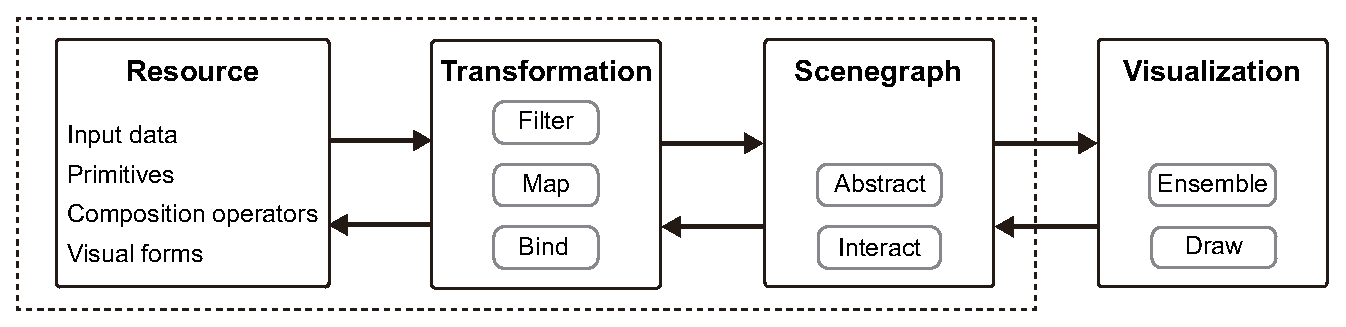
\includegraphics[width=0.98\linewidth]{images/composer.eps}
  \caption{The operational flowchart of the visualization composer.} \label{fg:flowchart}
\end{figure}

Conceptually, the final visualization is composed by three components: the visual form, construction component, the rendering code generation component, and the final production component.  In the first component, the visualization composer assembles  all elements of the Scenegraph module and the Transformation module, and generates a topological organization that describes the directed input-output links between elements. In the second component, the elements of each module are translated into JavaScript code. By solving conflicts between variable names and incorporating exception handling and other environment settings into the program, the production code is produced. The code can then be used for visualization and  interactive user modulation. The third component, compiles the produced code within the web browser using the evaluation function (eval) of JavaScript and displays the visualization.  The user can then search for errors and modify the results.


\subsection{Programmable Visualization Shaders}
We enable programmability by allowing the user to craft a piece of javascript code for each element of the Scenegraph module and the Transformation module. Specifically, the following schemes are employed to enable a visual programmable composition environment.

\noindent \textbf{The Visualization Shader:}  We denote a complete piece of custom built code as a \emph{visualization shader}.  Such a shader is used to create visual effects for specialized visualization elements. The effects achieved by visualization shaders are comprehensive, such as specifying visual properties, organizing graphical primitives, and designing a special visual form.  A visualization shader can be directly used to customize a visualization element and can be seamlessly integrated into the intermediate program that is generated by the system during the composition process.
When the composition process is completed, a set of javascript code associated with the Scenegraph and Transformation modules is synthesized and is run to generate a visualization.
We introduce three kinds of visualization shaders: expression, statement and block.
\begin{itemize}
  \item An \emph{Expression} is a mathematical or evaluation expression  that is used to set data binding operations (e.g.,  ``parent().width/4'' set a primitive's width to be a quarter of its parent). It refers to a control widget in the interface (see Figure~\ref{fg:interface} (e)).
  \item A \emph{Statement} is a set of algebraic functional equations to specify data transformation or visual mapping operations (e.g., ``normalized\_x=(x-min(x))/(max(x)-min(x))''). It refers to a control widget in the interface (see Figure~\ref{fg:interface} (f)).
  \item A \emph{block} denotes an editable function  with an input state and an output state. A block is shown and edited in a visual text editor (see Figure~\ref{fg:interface} (g)).   A bock-based shader offers the most flexible programmability, and can fulfill many kinds of special effects (e.g., a treemap layout algorithm).
\end{itemize}
%
%\begin{figure}[htb]
%  \includegraphics[width=0.98\linewidth]{images/shader.eps}
%  \caption{(a) An expression-based visualization shader; (b) A statement-based visualization shader; (c) A block-based visualization shader.} \label{fg:shader}
%\end{figure}


\noindent \textbf{Cross-module State Transfer:} To guarantee the user-generated program matches the associated elements and operations in composing a visualization, the states transferred from other module or inherited from other elements  can be exposed, used or modulated in a block-type shader.  We classify the states into three categories:
\begin{itemize}
  \item \noindent \textbf{The Input State} The input state denotes the custom built designs of elements in previous composition steps. It is  passed across four modules. The user can freely modulate an input state in writing a visualization shader. The input state is implicitly accessible if the user composes the visualization by direct manipulation in the Transformation, Scenegraph and the visualization modules.
  \item \noindent \textbf{The Output State} The modulated state in a visualization shader can be transferred to other visualization elements. The transfer can be specified in the shader, or specified by user interactions. The transferred state can be used for further transformation or bound to other visualization elements.
  \item
\noindent \textbf{The Global State} A global state is  instantiated when constructing the root node of the Scenegraphh and is used to specify functions (e.g., getCol: get a specific column of a table data) and global variables (e.g., the size of the visualization canvas).  The global state can be accessed by all elements during the customization of a visualization shader.
\end{itemize}


